\providecommand{\main}{..}
\documentclass[\main/TL_liquid.tex]{subfiles}
\graphicspath{{\main/images/}}
\setcounter{section}{2}
\begin{document}
\section{朝永-Luttinger模型}
\begin{frame}{ボソンフェルミオン対応}
    マヤ図形とYoung図形の対応関係から、Jacobiの三重積という不思議な式が現れることを見た。以降はこの対応関係が応用される例として、朝永-Luttinger模型について説明する。
\end{frame}

\begin{frame}{朝永-Luttinger模型}
    1次元のフェルミ粒子系を考える。基底状態からの低エネルギー励起においては、フェルミ運動量$k_F, -k_F$を基準にすることで、分散関係は
    \begin{align}
        \epsilon = \pm v_F k
    \end{align}
    と書ける。
    \begin{figure}[H]
        \centering
        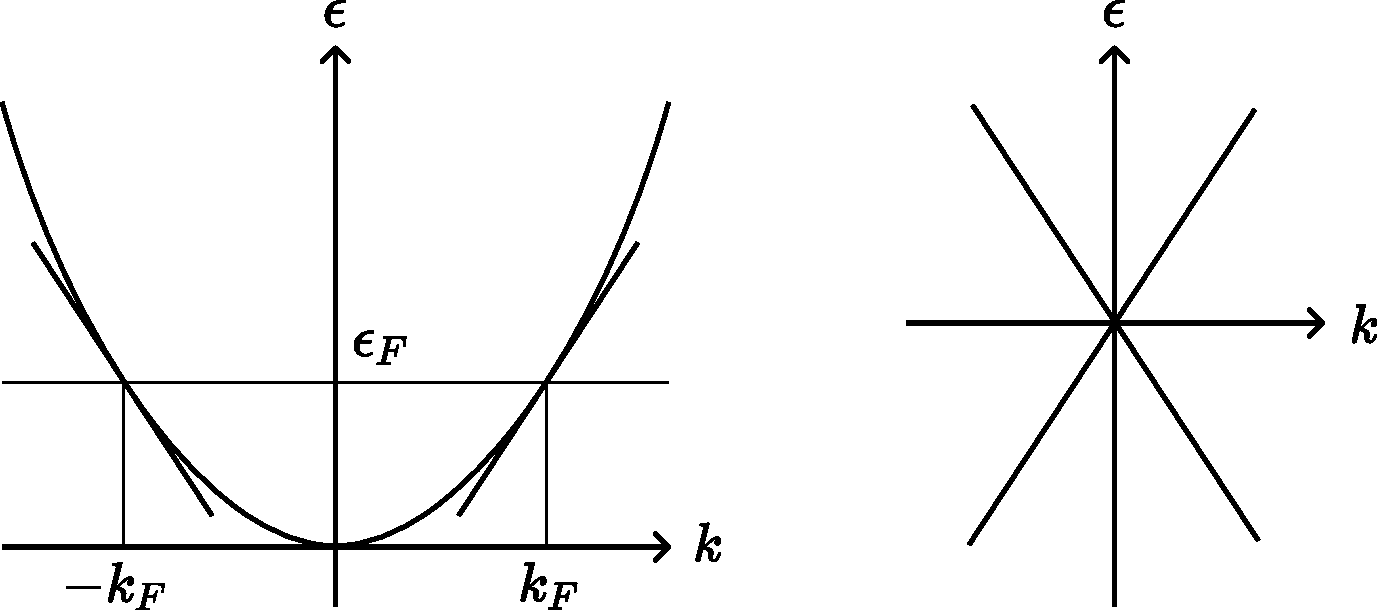
\includegraphics[scale = 0.3]{Tomonaga-Luttinger_model.pdf}
    \end{figure}
\end{frame}

\begin{frame}{朝永-Luttinger模型}
    朝永-Luttinger模型はフェルミ準位近くの低エネルギー励起をモデル化した模型で、
    ハミルトニアンの運動項は以下のように与えられる。
    \begin{align}
        H_0
        = \sum_{k \in \mathbb{Z}} k\qty[
            a_+^{\dagger}(k) a_+(k)
            - a_-^{\dagger}(k) a_-(k)
        ]
    \end{align}
    ただし、波数は整数値をとるように再定義した。またエネルギーの次元をもつ定数を掛けるべきだが、それも省略した。
    $a_{\pm}(k)$は以下の反交換関係を満たす。 
    \begin{gather}
        \{a_j(k),a_{j'}(k')\}
        = \{a_j^\dagger(k), a_{j'}^\dagger(k')\} = 0
        \\
        \{a_j(k),a_{j'}(k')\} = \delta_{j,j'}\delta_{k,k'}
    \end{gather}
    ただし、$j,j'$は$\pm$に値をとるとする。

    相互作用項については、後で述べる。
\end{frame}

\begin{frame}{電子とホール}
    基底状態において$k=0$までの準位が全て電子で埋められているとする。このとき、
    \begin{align}
        a_+(k) = \begin{cases}
            b_k & (k \ge 0) \\
            c_k^\dagger & (k < 0)
        \end{cases},
        \quad
        a_-(k) = \begin{cases}
            b_k & (k < 0) \\
            c_k^\dagger & (k \ge 0)
        \end{cases}
    \end{align}
    によって電子とホールの生成消滅演算子を定義すると、
    \begin{align}
        H_0 = \sum_k |k|(b_k^\dagger b_k + c_k^\dagger c_k) + W
    \end{align}
    となる。ただし、$W$は基底状態のエネルギーであり、以下のように与えられる。
    \begin{align}
        W = \sum_{k<0} k - \sum_{k \ge 0} k
    \end{align}
    これは負の無限大の量だが、定数だから気にしないことにする。
\end{frame}

% \begin{frame}{実空間表示}
%     \begin{align}
%         a_{\pm}(k) = \frac{1}{\sqrt{2\pi}} \int \dd{x} e^{ikx} \psi_{\pm}(x)
%     \end{align}
%     \begin{align}
%         H_0 = \int \dd{x} \qty[
%             \psi_+^\dagger(x)\qty(-i\dv{x})\psi_+(x)
%             - \psi_-^\dagger(x)\qty(-i\dv{x})\psi_-(x)
%         ]
%     \end{align}
% \end{frame}

\begin{frame}{ボソン化法}
    $H_0$に対する大分配関数は、$q = e^{-\beta}$としてJacobiの三重積(\ref{Jacobi triple product})を用いると、
    \begin{align}
        \Xi(\beta,0) = \prod_{k \in \mathbb{Z}}\qty(1+q^{|k|})^2 = \qty[\prod_{k=1}^\infty \frac{1}{1-q^k} \sum_{n \in \mathbb{Z}}q^{n(n+1)/2}]^2
    \end{align}
    となる。
    この式はフェルミオンフォック空間の中に、ボソンフォック空間が隠れていることを示唆している。
    これを具体的に構成してみよう。
\end{frame}

\begin{frame}{ボソン化法}
    密度演算子を以下のように定義する。
    \begin{align}
        \rho_+(p) &= \sum_k a_+^\dagger(k+p)a_+(k),
        \quad
        \rho_-(p) = \sum_k a_-^\dagger(k+p)a_-(k)
    \end{align}
    これらは交換関係
    \begin{align}
        &
        [\rho_+(p), \rho_-(p')] = 0
        \label{comm: RL}
        \\ &
        [\rho_+(-p), \rho_+(p')]
        = [\rho_-(p),\rho_-(-p')]
        = p\delta_{p,p'}
        \label{comm RR, LL}
    \end{align}
    を満たす (以降で計算する)。
    \begin{align}
        A_p = \frac{1}{\sqrt{p}} \rho_+(p), \quad
        A_p^\dagger = \frac{1}{\sqrt{p}} \rho_+(-p)
        \\
        B_p = \frac{1}{\sqrt{p}} \rho_-(-p), \quad
        B_p^\dagger = \frac{1}{\sqrt{p}}\rho_-(p)
    \end{align}
    と定義すれば、$A_p,A_p^\dagger,B_p,B_p^\dagger$はボソンの生成消滅演算子となる。
\end{frame}

\begin{frame}{交換関係}
    $p \ne p'$のとき、
    \begin{align}
        [\rho_+(-p),\rho_+(p')]
        &
        = \sum_{k,k'}\qty[a_+^\dagger(k-p)a_+(k),a_+^\dagger(k'+p') a_+(k')]
    \end{align}
    となる。これは、
    \begin{align}
        [AB,CD] &= A[B,CD] + [A,CD]B
        \\ &
        = A\{B,C\}D - AC\{D,B\} + \{A,C\}DB - C \{D,A\}B
    \end{align}
    から、
    \begin{align}
        [\rho_+(-p),\rho_+(p')]
        &
        = \sum_{k \in \mathbb{Z}} a_+^\dagger(k-p) a_+(k-p')
        \\ & \quad\quad
        - \sum_{k \in \mathbb{Z}} a_+^\dagger(k-p+p') a_+(k)
        = 0
    \end{align} 
    と計算できる。
\end{frame}

\begin{frame}{交換関係}
    同様に、$p=p'$のとき、
    \begin{align}
        [\rho_+(-p),\rho_+(p)]
        &
        = \sum_{k \in \mathbb{Z}} \qty(a_+^\dagger(k-p) a_+(k-p)-a_+^\dagger(k)a_+(k))
    \end{align}
    であるが、\alert{これはゼロにはならない!}

    任意の状態ベクトルに対して、
    \begin{align}
        \sum_{k \in \mathbb{Z}} a_+^\dagger(k-p) a_+(k-p),
        \quad
        \sum_{k \in \mathbb{Z}} a_+^\dagger(k)a_+(k)
    \end{align}
    を作用させると、
    フェルミの海に無限に粒子が詰まっていることから、
    状態ベクトルは発散してしまう。
    このことから項を足し上げる順序を安易に変えてはいけないことが分かる。
\end{frame}

\begin{frame}{交換関係}
    状態空間の中で$k \le k_0$の準位が完全に占有されているような部分空間を考える。このとき、
    \begin{align}
        [\rho_+(-p),\rho_+(p)]
        &=
        \sum_k \qty(n_+(k-p) - n_+(k))
        \\ & \nonumber
        = \qty[\sum_{k \le k_0} + \sum_{k _0 < k}] \qty(n_+(k-p)-n_+(k))
        \\ & \nonumber
        = \sum_{k_0 < k} \qty(n_+(k-p) - n_+(k))
        \\ &
        = \sum_{k_0 < k \le k_0+p} n_+(k-p)
        = p
    \end{align}
    となる。結果は$p_0$に依存しないので、$p_0 \to -\infty$とできる。
    $\rho_-(p)$についても同様に計算することで、(\ref{comm RR, LL})が成り立つことが分かる。
\end{frame}

\begin{frame}{交換関係}
    つぎに、密度演算子とハミルトニアンの交換関係を計算する。
    \begin{align}
        [H_0, \rho_{\pm}(p)] &
        = \nonumber
        \pm \sum_{k,k'} k\qty[a_{\pm}^\dagger(k)a_{\pm}(k),a_{\pm}^\dagger(k'+p)a_{\pm}(k')]
        \\ &\nonumber
        = \pm \sum_k k \qty(a_{\pm}^\dagger(k) a_{\pm}(k-p)-a_{\pm}^\dagger(k+p)a_{\pm}(k))
        \\ &\nonumber
        = p\sum_k a_{\pm}^\dagger(k) a_{\pm}(k-p)
        \\ &
        = \pm p \rho_{\pm}(p)
    \end{align}
    よって
    \begin{align}
        [H_0, A_p] = p A_p,
        \quad
        [H_0, B_p] = p B_p
    \end{align}
    となる。
\end{frame}

\begin{frame}{ハミルトニアンの書き換え}
    交換関係から、
    \begin{align}
        H_0 = \sum_{p>0} p(A_p^\dagger A_p + B_p^\dagger B_p)
    \end{align}
    と表せそう。実際は、
    \begin{align}
        H_0 = \sum_{p>0} p(A_p^\dagger A_p + B_p^\dagger B_p) + \frac{1}{2}Q_+(Q_++1) + \frac{1}{2}Q_-(Q_--1)
        \label{Bosoinzation Hamiltoninan}
    \end{align}
    となる。ただし、
    \begin{align}
        Q_+ = \sum_{k \ge 0} b_k^\dagger b_k - \sum_{k<0} c_k^\dagger c_k,
        \quad
        Q_- = \sum_{k < 0} b_k^\dagger b_k - \sum_{k \ge 0} c_k^\dagger c_k
    \end{align}
    である。
    $Q_{\pm} = \sum_k a_{\pm}^\dagger(k)a_{\pm}(k) + \mathrm{const.}$から、
    $A_p, B_p$が$Q_{\pm}$と交換することが分かる。
\end{frame}

\begin{frame}{ハミルトニアンの書き換え}
    $A_p, B_p$が$Q_{\pm}$の固有値を変化させないことから、
    状態空間を$Q_+, Q_-$の固有空間に分けることにする。
    基底状態$\ket{\Omega_{m,n}}$を
    \begin{align}
        Q_+ \ket{\Omega_{m,n}} = m,
        \quad
        Q_- \ket{\Omega_{m,n}} = n
    \end{align}
    および
    \begin{align}
        A_p \ket{\Omega_{m,n}} = B_p \ket{\Omega_{m,n}} = 0
    \end{align}
    によって定義する。
    $Q_+,Q_-$の固有値が$m,n$であるような状態は
    $\ket{\Omega_{m,n}}$に$A_p^\dagger, B_p^\dagger$を掛けていくことで得られる。
\end{frame}

\begin{frame}{ハミルトニアンの書き換え}
    基底状態は、以下のマヤ図形で表される。
    \begin{figure}[H]
        \centering
        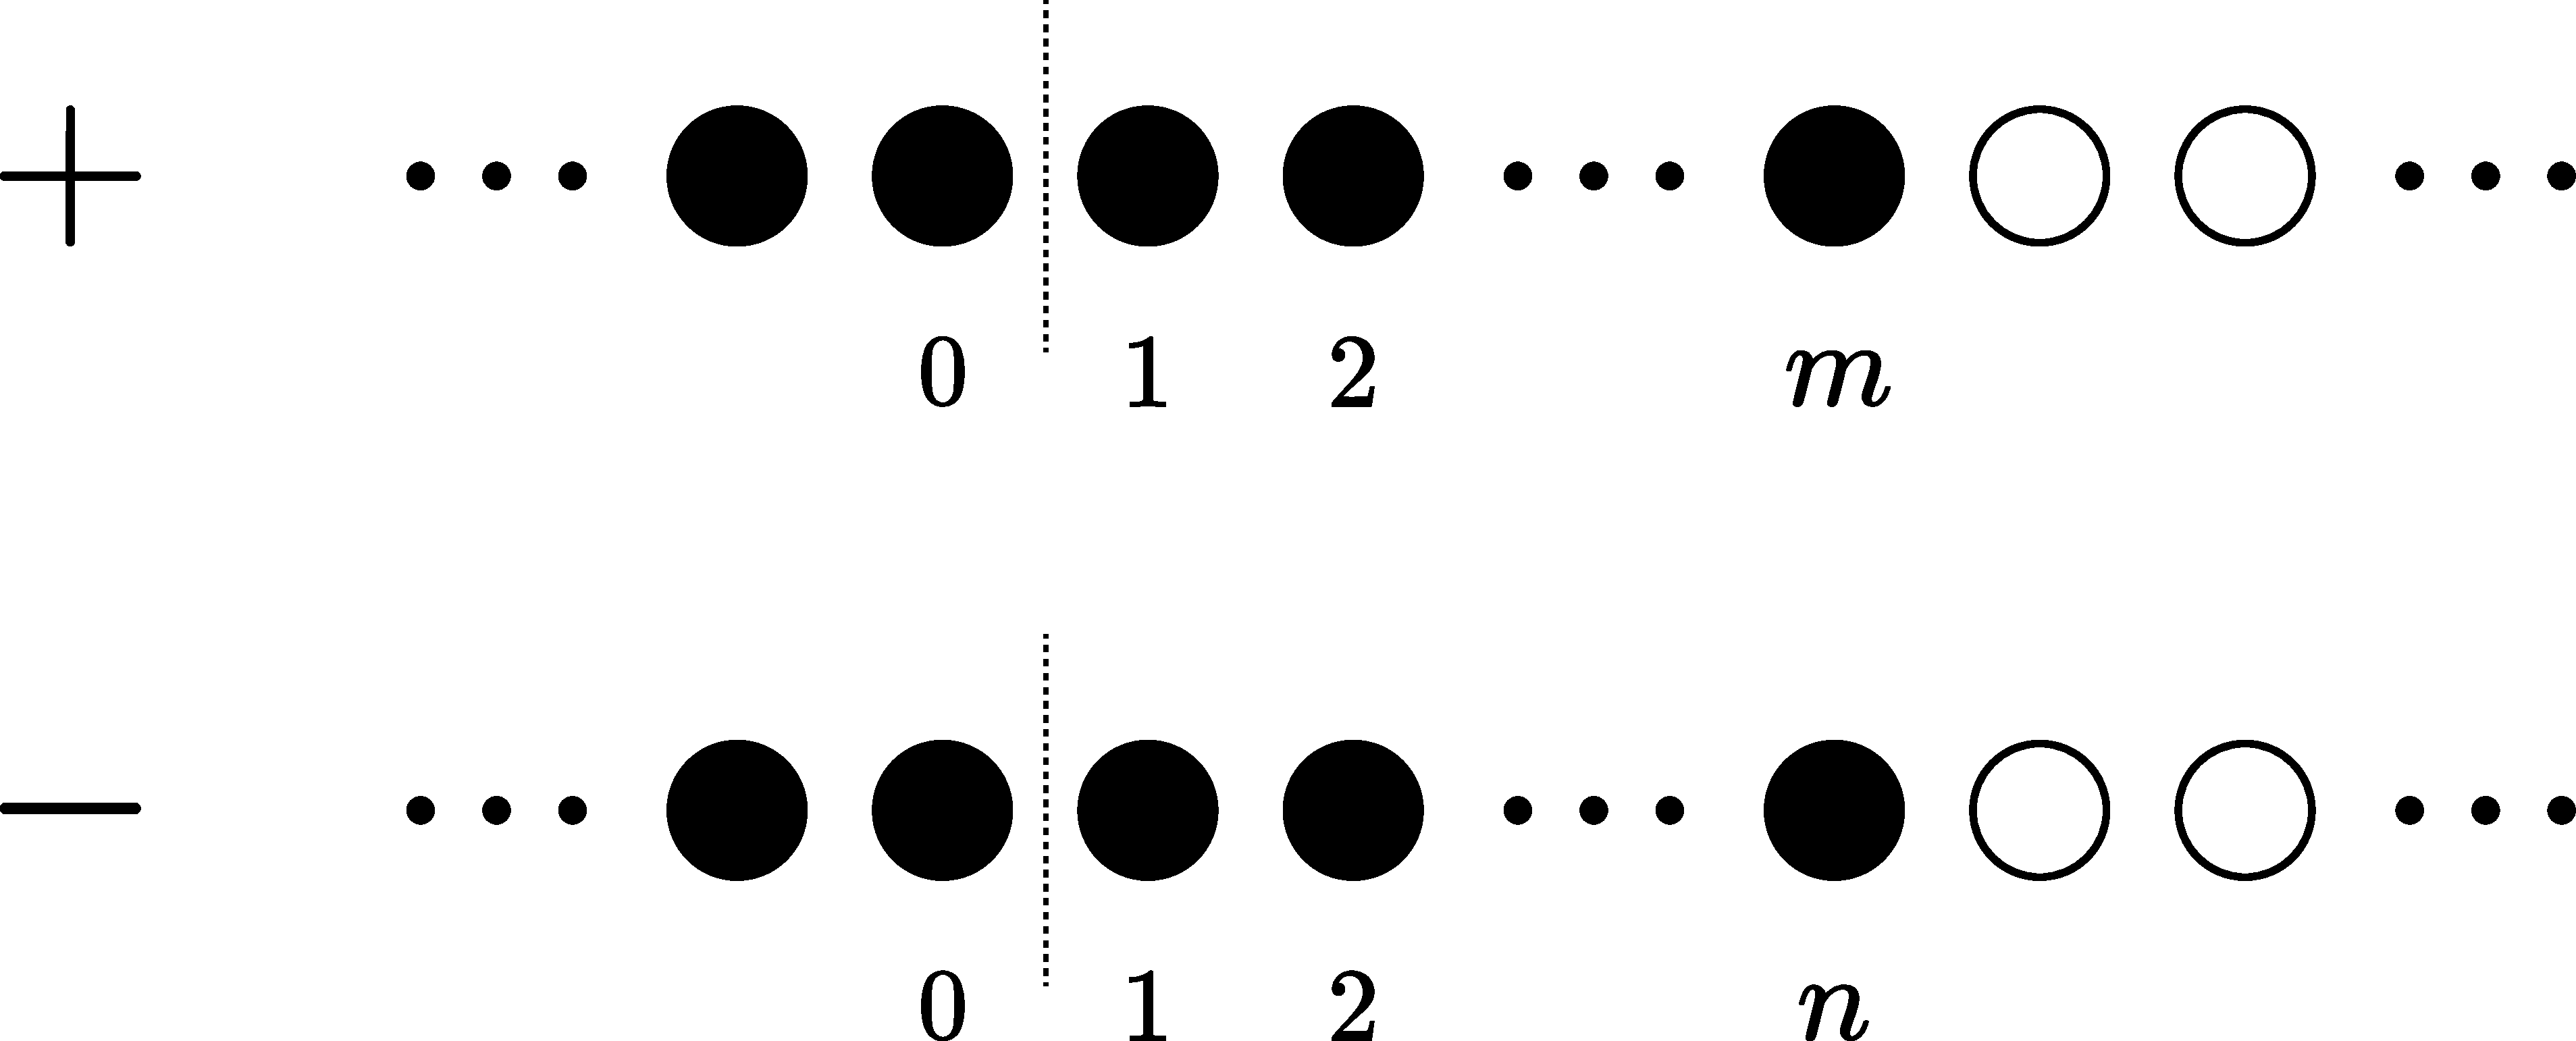
\includegraphics[scale = 0.1]{TL_gnd.pdf}
    \end{figure}
    よって基底状態のエネルギーは (真空のエネルギーを除いて)、
    \begin{align}
        \mel{\Omega_{m,n}}{H_0}{\Omega_{m,n}}
        = \frac{1}{2}m(m+1) + \frac{1}{2}n(n-1)
    \end{align}
    となる。したがって、(\ref{Bosoinzation Hamiltoninan})が成り立つことが分かる。
\end{frame}

\begin{frame}{相互作用項}
    次に、以下のような相互作用項を考える。
    \begin{align}
        H_{\mathrm{int}}
        = \frac{1}{2\pi} \sum_{p>0} pV(p)(
            A_p^\dagger A_p + B_p B_p^\dagger
            + A_p^\dagger B_p^\dagger + A_p B_p
        )
    \end{align}
    フェルミオン演算子で書くと、
    \begin{align}
        A_p^\dagger A_p
        = \sum_{k,k' \in \mathbb{Z}}
            a_+^\dagger(k-p) a_+(k) a_+^\dagger(k'+p) a_+(k')
        \\
        B_p B_p^\dagger
        = \sum_{k,k' \in \mathbb{Z}}
            a_-^\dagger(k-p) a_-(k) a_-^\dagger(k'+p) a_-(k')
        \\
        A_p^\dagger B_p^\dagger
        = \sum_{k,k' \in \mathbb{Z}}
            a_+^\dagger(k-p)a_+(k) a_-^\dagger(k'+p)a_-(k')
        \\
        A_p B_p
        = \sum_{k,k' \in \mathbb{Z}}
            a_+^\dagger(k+p)a_+(k) a_-^\dagger(k'-p)a_-(k')
    \end{align}
\end{frame}

\begin{frame}{Bogoliubov変換}
    ハミルトニアンを対角化するために,Bogoliubov変換
    \begin{align}
        \mqty(\alpha_p\\ \beta_p^\dagger) =
        \mqty(
            \cosh \theta_p & \sinh \theta_p \\
            \sinh\theta_p & \cosh \theta_p
        )
        \mqty(A_p\\B_{p}^\dagger)
        \label{Bogoliubov transformation}
    \end{align}
    を用いる.$\theta_p$は後で求めるとして,まずこの変換の性質について述べておく.
    変換行列を$U(\theta_p)$とおくと,これは明らかにエルミートである.また$\theta$に関する加法性
    \begin{align}
        U(\theta)U(\theta') = U(\theta + \theta')
    \end{align}
    が成り立つ.$U(0) = I$であるから$U(-\theta) = U(\theta)^{-1}$である.さらに,
    \begin{align}
        \eta U(\theta) \eta = U(-\theta) = U(\theta)^{-1}, \quad \eta = \mqty(1&0\\0&-1)
    \end{align}
    が分かる.
\end{frame}

\begin{frame}{Bogoliubov変換}
    ここで,
    \begin{align}
        \mqty(
            [A,C] & [A,D] \\ 
            [B,C] & [B,D]
            )
        = \qty[\mqty(A\\B)\mqty(C&D)]
    \end{align}
    という表記を導入しよう.すると,
    \begin{align}
        \qty[\mqty(\alpha_p\\ \beta_p^\dagger)\mqty(\alpha_{p'}^\dagger & \beta_{p'})]
        &\nonumber
        =
        U\qty[\mqty(A_p\\ B_p^\dagger)\mqty(A_{p'}^\dagger & B_{p'})]U
        \\ &\nonumber
        = \delta_{p,p'}U \eta U
        = \delta_{p,p'} U\eta U \eta \eta
        \\ &
        = \delta_{p,p'}\eta
    \end{align}
    となる.すなわち
    \begin{gather}
        [\alpha_{p}, \alpha_{p'}^\dagger] = [\beta_{p}, 
        \beta_{p'}^\dagger] = \delta_{p,p'},
        \\
        [\alpha_{p},\beta_{p'}] = [\alpha_{p}^\dagger, \beta_{p'}^\dagger] = 0
    \end{gather}
    となる.その他の交換関係は明らかにゼロになるから,\alert{Bogoliubov変換は交換関係を保つ}.
\end{frame}

\begin{frame}{Bogoliubov変換}
    ここで、
    \begin{align}
        & \nonumber
        \mqty(A_p^\dagger & B_p)
        \mqty(
            p + pV(p)/2\pi & pV(p)/2\pi
            \\
            pV(p)/2\pi & p + pV(p)/2\pi
        )
        \mqty(A_p \\ B_p^\dagger)
        \\ & \nonumber
        = E_p\mqty(A_p^\dagger & B_p)U(2\theta_p)
            \mqty(A_p \\ B_p^\dagger) 
        \\ & \nonumber
        = E_p\mqty(A_p^\dagger & B_p)U^\dagger(\theta_p) U(\theta_p)
        \mqty(A_p \\ B_p^\dagger) 
        \\ &
        = E_p(\alpha_p^\dagger \alpha_p + \beta_p \beta_p^\dagger)
    \end{align}
    と書ける。ただし、
    \begin{align}
        E_p = p\sqrt{1 + \frac{V(p)}{\pi}},
        \quad
        \tanh(2\theta_p) = \frac{V(p)}{V(p)+2\pi}
    \end{align}
    である。
\end{frame}

\begin{frame}{Bogoliubov変換}
    したがって、ハミルトニアンは
    \begin{align}
        &
        H = \sum_{p>0} E_p(\alpha_p^\dagger \alpha_p + \beta_p^\dagger \beta_p) + E_0(Q_+, Q_-)
        \\ &
        E_0
        = \sum_{p>0}(E_p - p)
            + \frac{1}{2}Q_+(Q_++1)
            + \frac{1}{2}Q_-(Q_--1)
    \end{align}
    と対角化される。$E_p - p$は$B_p^\dagger B_p,~ \beta_p \beta_p^\dagger$の順序を入れ替えるときに出てくる補正である。
\end{frame}
% \begin{frame}{基底状態}
    
% \end{frame}
\end{document}